\documentclass[a4paper,12pt]{article}

% \usepackage{array}
% \usepackage{tabularx}
% \usepackage{multirow}
% \usepackage{longtable}
% \usepackage{enumitem}

% \usepackage{color}
% \usepackage{graphicx}
% \usepackage{float}
\usepackage{tikz}

\usepackage{amsmath}
\usepackage{amssymb}
% \usepackage{mathtools}
% \usepackage{calc}

% \usepackage{listings}
% \usepackage{minted}

\usepackage[fontset=none]{ctex}
\usepackage{fontspec}
\usepackage{xeCJK}
\usepackage[english]{babel}

\usepackage{hyperref}

\setCJKmainfont[Path="../Assets/Fonts/SourceHan/Serif/",BoldFont={SourceHanSerifSC-Bold.otf},AutoFakeSlant=0.25]{SourceHanSerifSC-Regular.otf}
\setCJKsansfont[Path="../Assets/Fonts/SourceHan/Sans/",BoldFont={SourceHanSansSC-Bold.otf},AutoFakeSlant=0.25]{SourceHanSansSC-Regular.otf}
\setCJKmonofont[Path="../Assets/Fonts/SourceHan/Mono/"]{SourceHanMono.ttc}
\newCJKfontfamily\kaiti[Path="../Assets/Fonts/AR_PL_UKai/"]{ukai.ttc}

\title{Assignment-1}
\author{刘行逸}
\date{20250916}

\hypersetup{
    pdftitle={Assignment-1},
    pdfauthor={刘行逸},
}

\begin{document}
\maketitle

\section*{1}
\addcontentsline{toc}{section}{1}
\begin{align*}
    \begin{vmatrix}
        1 \\
    \end{vmatrix}         & = 1 > 0                                                          \\
    \begin{vmatrix}
        1      & \alpha \\
        \alpha & 4      \\
    \end{vmatrix}      & = 4 - \alpha^2 > 0, \ \alpha \in (-2, 2)                            \\
    \begin{vmatrix}
        1      & \alpha & -1 \\
        \alpha & 4      & 2  \\
        -1     & 2      & 4  \\
    \end{vmatrix} & = 1 \times 4 \times 4 + (-1) \times 2 \alpha + (-1) \times 2 \alpha      \\
                            & - (-1) \times 4 \times (-1) - 4 \alpha^2 - 1 \times 2 \times 2 \\
                            & = -4 \alpha^2 - 4 \alpha + 8                                   \\
                            & = -4 (\alpha^2 + \alpha -2) > 0, \ \alpha \in (-2, 1)          \\
    \\
    \therefore \alpha       & \in (-2, 1)                                                    \\
\end{align*}

\section*{2}
\addcontentsline{toc}{section}{2}
\subsection*{(a)}
\addcontentsline{toc}{subsection}{(a)}
\begin{center}
    \begin{minipage}{0.525\textwidth}
        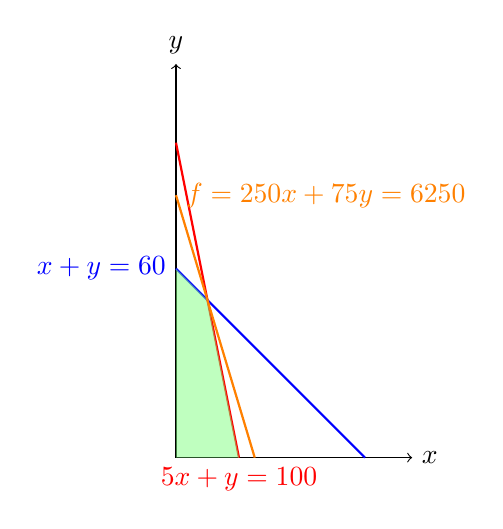
\begin{tikzpicture}[scale=0.04]
            \draw[->] (0,0) -- (75,0)node[right]{$x$};
            \draw[->] (0,0) -- (0,125)node[above]{$y$};

            \draw[thick,red] (20,0)node[below]{$5 x + y = 100$} -- (0,100);
            \draw[thick,blue] (60,0) -- (0,60)node[left]{$x + y = 60$};

            \fill[green!50,opacity=0.5] (0,0) -- (20,0) -- (10,50) -- (0,60) -- cycle;

            \draw[thick,orange] (25,0) -- (0,250/3)node[right]{$f = 250 x + 75 y = 6250$};
        \end{tikzpicture}
    \end{minipage}
    \hfill
    \begin{minipage}{0.425\textwidth}
        \begin{align*}
            x = 10, \ y & = 50,                          \\
            \max{f}     & = 250 \times 10 + 75 \times 50 \\
                        & = 6250                         \\
        \end{align*}
    \end{minipage}
\end{center}

\subsection*{(b)}
\addcontentsline{toc}{subsection}{(b)}
\begin{center}
    \begin{minipage}{0.525\textwidth}
        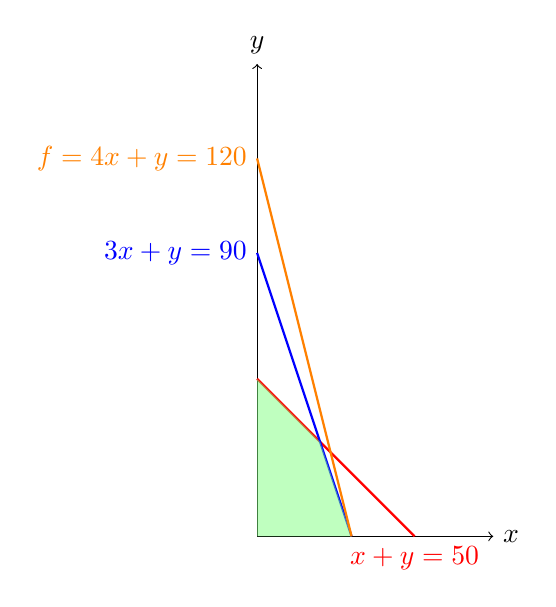
\begin{tikzpicture}[scale=0.04]
            \draw[->] (0,0) -- (75,0)node[right]{$x$};
            \draw[->] (0,0) -- (0,150)node[above]{$y$};

            \draw[thick,red] (50,0)node[below]{$x + y = 50$} -- (0,50);
            \draw[thick,blue] (30,0) -- (0,90)node[left]{$3 x + y = 90$};

            \fill[green!50,opacity=0.5] (0,0) -- (30,0) -- (20,30) -- (0,50) -- cycle;

            \draw[thick,orange] (30,0) -- (0,120)node[left]{$f = 4 x + y = 120$};
        \end{tikzpicture}
    \end{minipage}
    \hfill
    \begin{minipage}{0.425\textwidth}
        \begin{align*}
            x = 30, \ y & = 0,              \\
            \max{f}     & = 4 \times 30 + 0 \\
                        & = 120             \\
        \end{align*}
    \end{minipage}
\end{center}

\section*{3}
\addcontentsline{toc}{section}{3}
\begin{align*}
    \text{minimize} & \quad f = 5 x + 7 y \\
    \text{s.t.}     & \quad
    \begin{cases}
        2 x + y & \geq 8  \\
        x + 2 y & \geq 10 \\
        x, y    & \geq 0  \\
    \end{cases}
\end{align*}

\section*{4}
\addcontentsline{toc}{section}{4}
\begin{align*}
    \text{minimize} & \quad f = (16, 10, 15, 10, 12, 10) (x_{P, A}, x_{P, B}, x_{P, C}, x_{Q, A}, x_{Q, B}, x_{Q, C})^T \\
    \text{s.t.}     & \quad
    \begin{cases}
        x_{P,A} + x_{Q,A}                                    & \geq 5 \\
        x_{P,B} + x_{Q,B}                                    & \geq 5 \\
        x_{P,C} + x_{Q,C}                                    & \geq 4 \\
        x_{P,A} + x_{P,B} + x_{P,C}                          & \leq 8 \\
        x_{Q,A} + x_{Q,B} + x_{Q,C}                          & \leq 6 \\
        x_{P,A}, x_{P,B}, x_{P,C}, x_{Q,A}, x_{Q,B}, x_{Q,C} & \geq 0 \\
    \end{cases}
\end{align*}

\end{document}
